\section{Globales FEM}
Wie in der Aufgabenstellung beschrieben, soll zur Überprüfung der Handrechnungen ein gloables FEM-Modell zur Anwendung kommen. In diesem Kapitel wird nun beschrieben, wie dieses FEM-Modell aufgesetzt und welche Annahmen getroffen werden. Weiter werden die Resultate der Simulationen aufgeführt, mit den Handrechnungen verglichen und beurteilt.\\

Mit dem globalen FEM-Modell sollen folgende Punkte bestimmt werden:
\begin{itemize}
  \item Lagerreaktionen
  \item Maximale Axialkräfte, Querkräfte und Biegemomente in Chassis, Dach und derTrägern A und B
  \item Kontaktreaktion: Chassis zu Träger A und B
  \item Kontaktreaktion: Chassis zu Boden
\end{itemize}

Ebenfalls wird das Verformungsverhalten genauer betrachtet um kritische Verformungen feststellen zu können und die Konstruktion entsprechend anpassen zu können.

\subsection{Idealisierung und Modell}
Das FEM-Modell des Solar Butterflys wird aus Balken und Schalenkörper aufgebaut. Das Chassis, die Träger A und B sowie die Dachträger werden als Balken mit den entsprechenden Querschnitten modeliert. Die Wände, Dächer und der Boden werden das Schalenkörper modelliert, wobei den Schalenkörper jeweils ein Lagenaufbau zugewiesen wird, welcher die Sandwichbauweise nachstellt. In den Abbildungen \ref{FEM Mesh1} ist das komplette Modell des Solar Butterflys zu sehen. In der Abbildung \ref{FEM Mesh3} wurden die Schalenkörper ausgeblendet, sodass nur die Balken sichtbar sind.

\begin{figure}[ht!]
  \centering
  \centering
  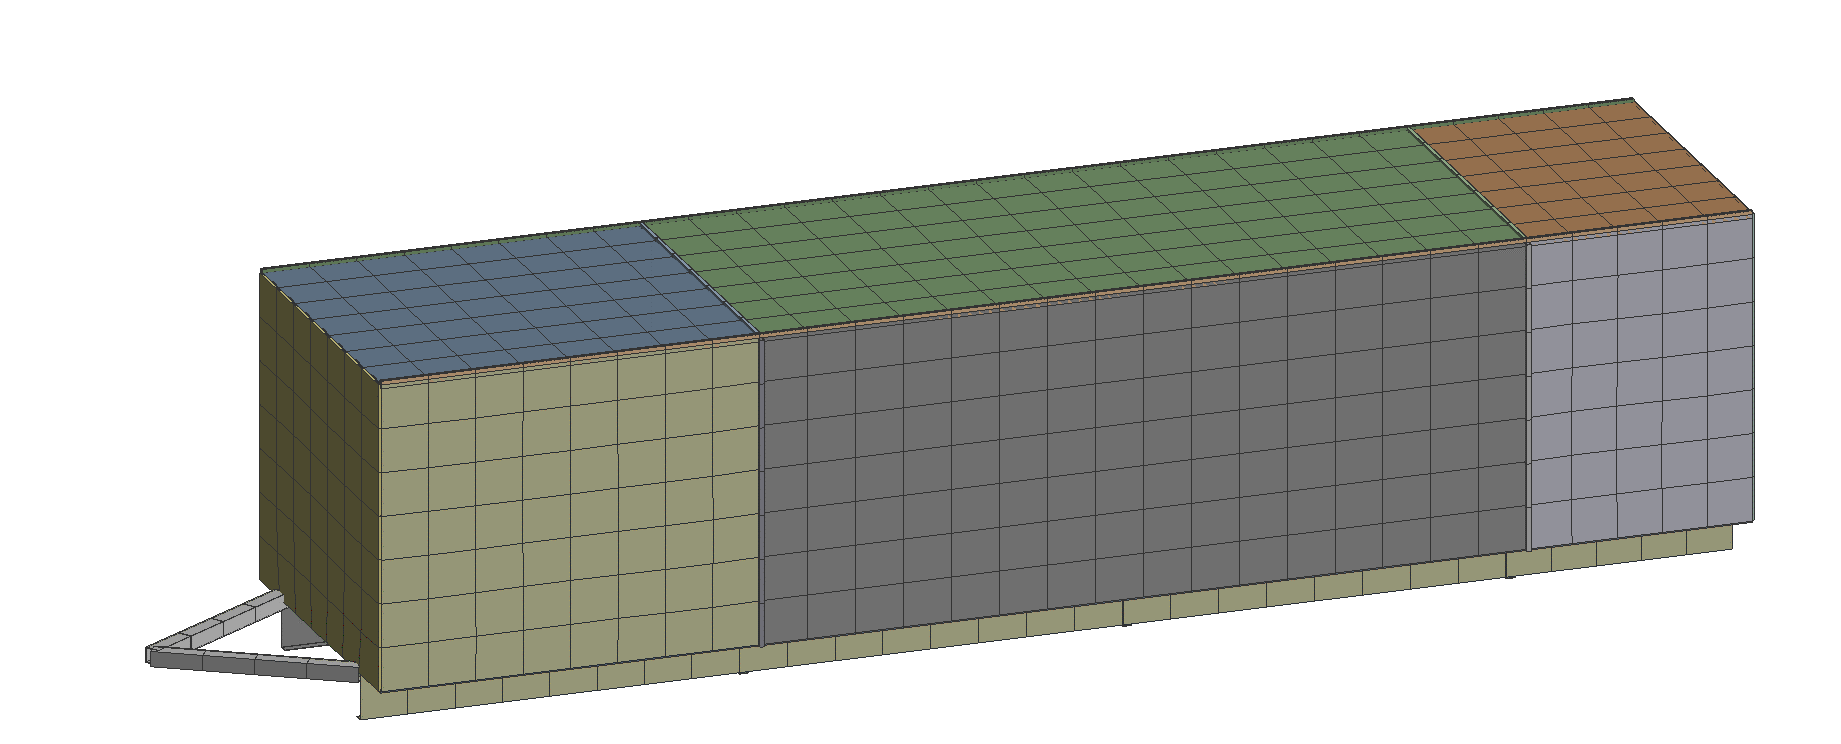
\includegraphics[width=.7\linewidth]{04_figures/FEM Mesh1.png}
  \caption{Darstellung der Balken und Schalenkörper im FEM-Modell}
  \label{FEM Mesh1}
\end{figure}
\begin{figure}[ht!]
  \centering
  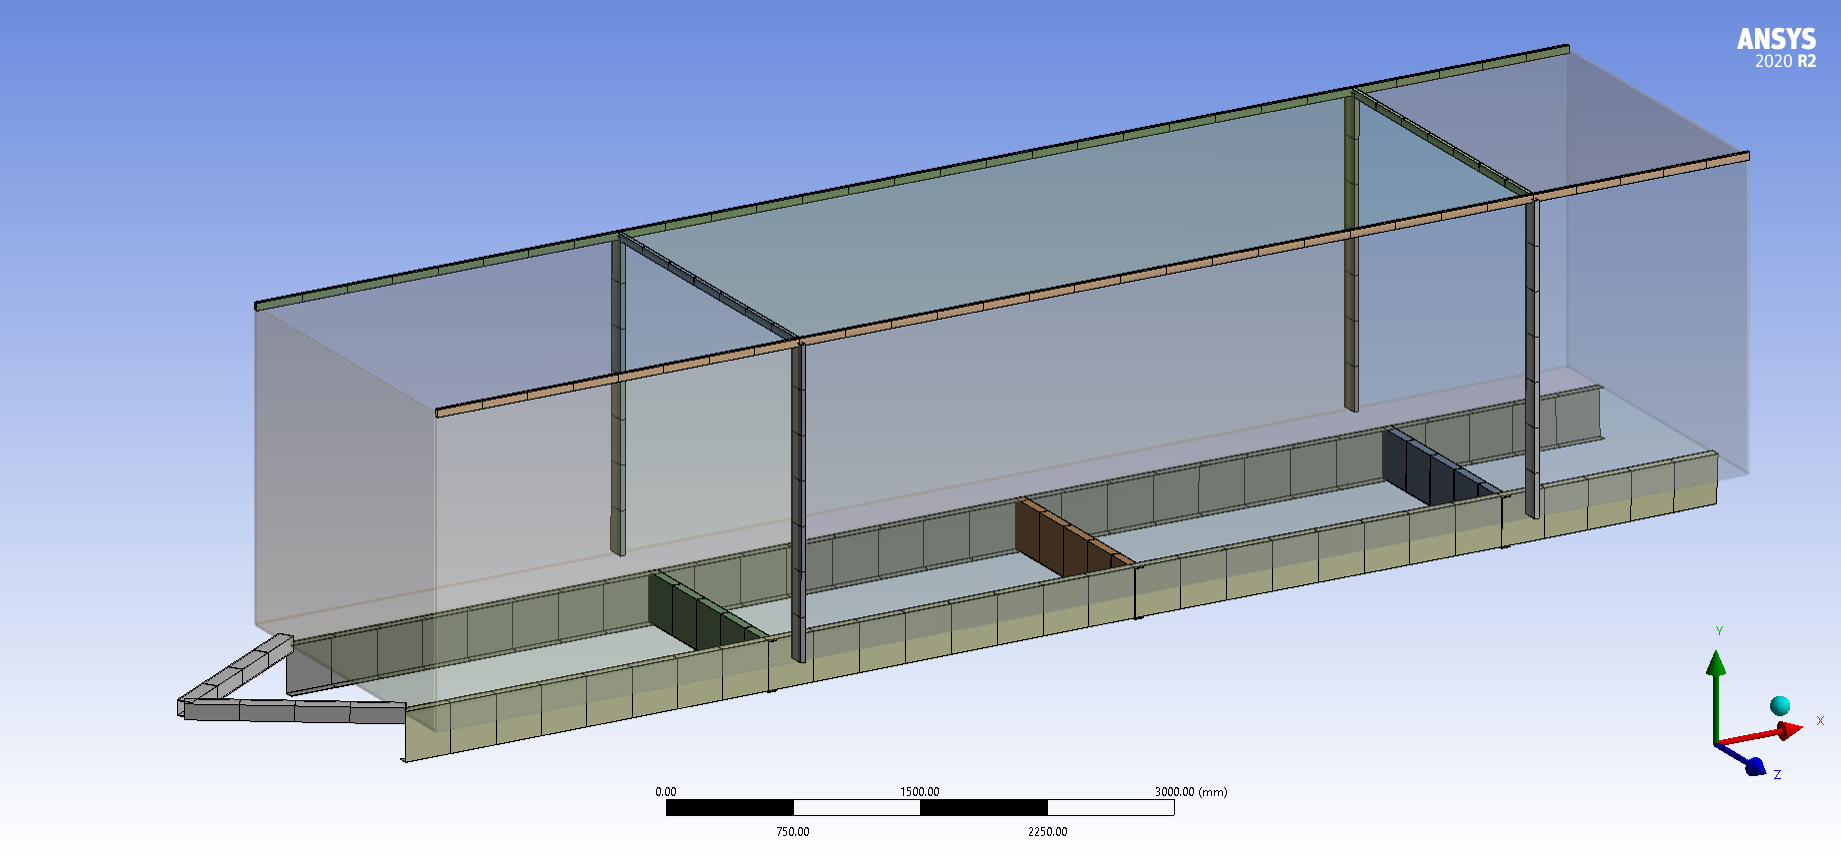
\includegraphics[width=.7\linewidth]{04_figures/FEM Mesh3.png}
  \caption{Darstellung der als Balken idealisierten Körper}
  \label{FEM Mesh3}
\end{figure}

Um die Masse des Solar Butterflys modellieren zu können, werden, zusätzlich zu den Massen der modellierten Bauteilen, Punktmassen (Point-mass) eingeführt. Es werden für die drei Raumelemente Küche, Mittelkörper und Bad je eine Punktmasse definiert, deren Masse und Trägheitsmomente mit der Hilfe der Massenverteilung aus dem Kapitel KAPITEL bestimmt werden. In der Abbildung \ref{img:FEM Punktmasse} sind die Verbindung der Punktmassen mit dem Rest des Modelles dargestellt.\\
\begin{figure}[h]
  \centering
  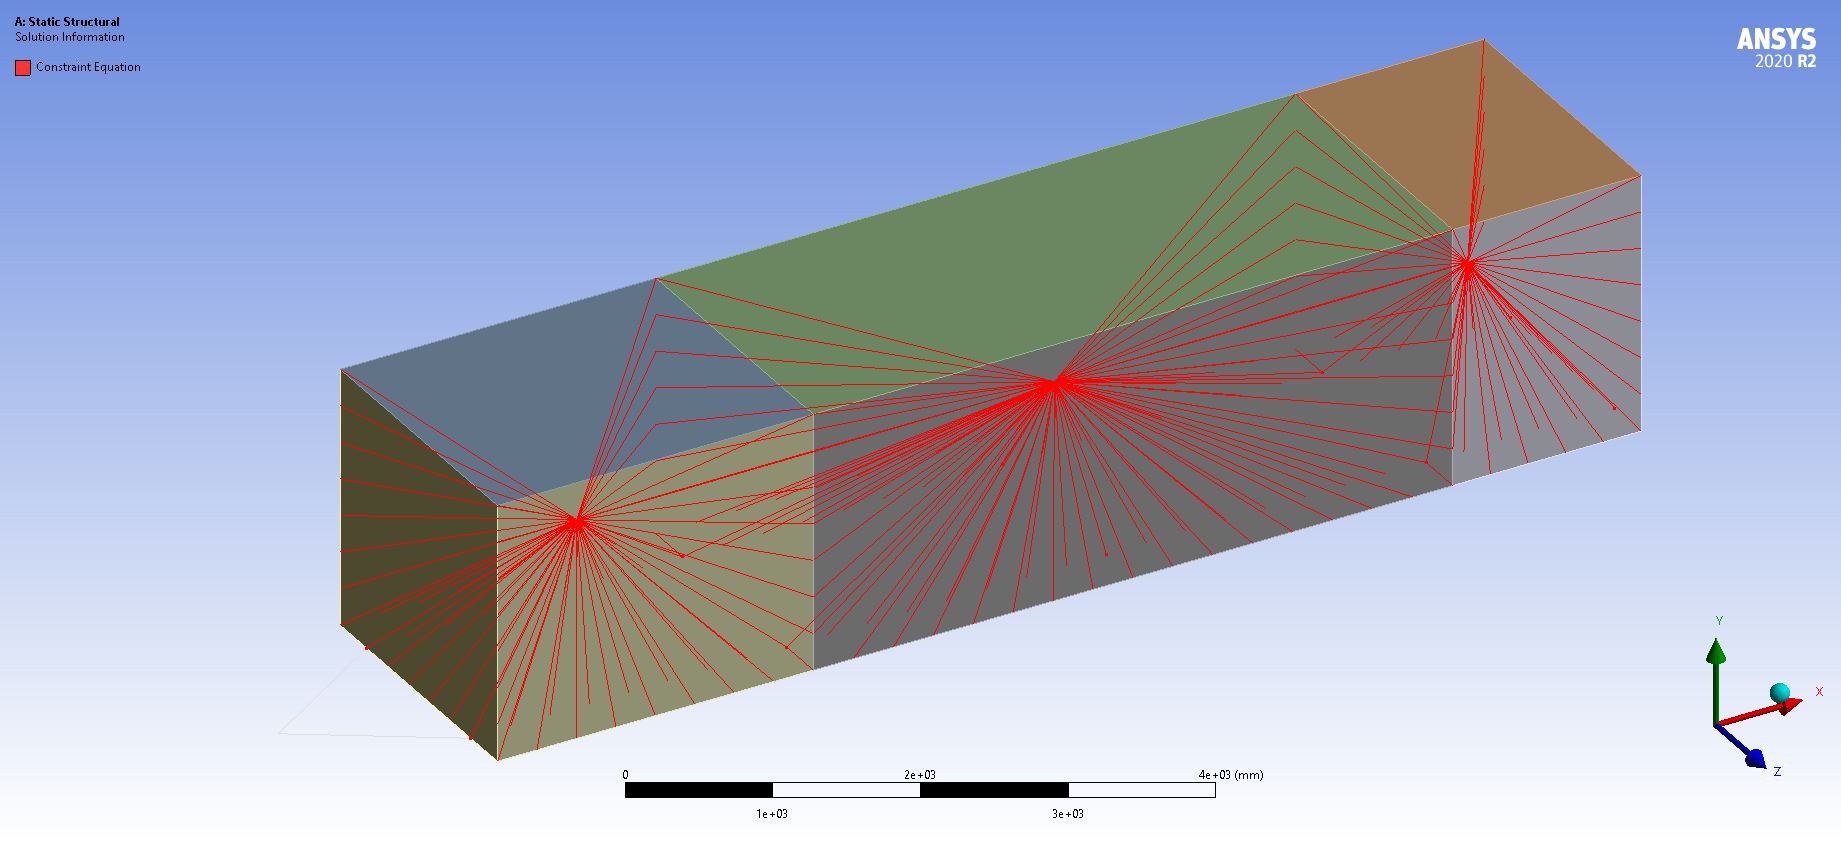
\includegraphics[width=0.7\linewidth]{04_Figures/FEM Punktmasse.png}
  \caption{Verbindungen der Punktmassen zum Rest des Modelles}
  \label{img:FEM Punktmasse}
\end{figure}

Die Deichsel, Längsträger und Querträger des Chassis werden durch das Zusammenführen der deckungsgleichen Koten miteinander verbunden. Auf die selbe Art und Weise werden die Träger A und B, die Träger des Daches sowie der Boden, die Wände und das Dach des Aufbaus miteinander verbunden. Der nun verbundene Aufbau wiederum wird auf zwei Arten mit dem Chassis verbunden. Einerseits werden die Träger A und B über Fixe MPC-Kontakte (alle Freiheitsgrade eingeschränkt) an ihrem untersten Knoten mit dem Chassis verbunden. Weiter wird der Boden über Translatorische MPC Kontakte mit den Längsträgern des Chassis verbunden. Sie räpresentieren die Klebestellen zwischen Boden und Chassis. Mit dem Auslesen dieser beiden Kontaktreaktionen können Aussagen bezüglich der Klebestelle zwischen Chassis und Boden, sowie auch die über die Verbindung zwischen den Trägern A und B und dem Chassis gemacht werden.\\
In allen folgenden FEM-Simulationen ist der Solar Butterfly analog zu den Berechnungen im Kapitel \ref{sub:Longitudinale Beschleunigung} (Lastfall \emph{1.1 Vertikale Beschleunigung}) gelagert. Am Spitz der Deichsel sind die rotatorischen Freiheitsgrade freigegeben, die translatorischen jedoch eingeschränkt. An der Achse wird lediglich die Verschiebung in x-Richtung (Fahrtrichtung) zugelassen.


\subsubsection{Vertikale Beschleunigung}
Die Tabelle \ref{tab:FEM 1.1} stellt eine Zusammenstellung der Resultate zur FEM-Simulation des Lastfalles \emph{1.1 Vertikale Beschleunigung} dar. Die Schnittkräfte und Kontaktreaktionen beziehen sich jeweils auf einen einzelnen Balken oder Verbindungsstelle. Die Kontaktreaktion zwischen Chassis und Boden bezieht sich auf eine einzelne Knotenverbindung. Insgesammt ist der Boden an jedem Längsträger an 30 Stellen verbunden. Über die Gurtenfläche pro Abschnitt des Chassis kann auf die Spannungen in der Verbindung geschlossen werden.\\
Bei einer Fläche von 17880 $mm^2$ pro Abschnitt ergibt sich eine maximale Normalspannung von 0.04 MPa und eine maximale Schubspannung von 0.54 MPa. Beide Werte liegen deutlich unterhalb des Design-Allowable. Hierbei muss jedoch angemerkt werden, dass lokal die Spannungen deutlich höher liegen könnten und, dass das verwendete Modell nicht geeignet ist um diese Spannungskonzentrationen zu erkennen.


\begin{table}[H]
\centering
\begin{tabular}{lcccccc}
Grösse	&	Einheit	&	x	&	y	&	z	&	Total	&	Berechnet	\\	\hline
\multicolumn{5}{l}{\textbf{Lagerreaktionen}}									&		&		\\	\thickhline
Deichsel	&	N	&	0	&	3193	&	0	&	3193	&	-1028	\\
Chassis Links	&	N	&	0	&	35171	&	6733	&	35810	&	37300	\\
Chassis Rechts	&	N	&	0	&	35171	&	-6733	&	35810	&	37300	\\	\hline	\\
\multicolumn{5}{l}{\textbf{Chassis}}									&		&		\\	\thickhline
Axialkraft	&	N	&		&		&		&	-50730	&	-44518	\\
Querkraft	&	N	&		&		&		&	17003	&	19079	\footnotemark \\
Biegemoment	&	kNmm	&		&		&		&	16980	&		\\	\hline	\\
\multicolumn{5}{l}{\textbf{Dach}}									&		&		\\	\thickhline
Axialkraft	&	N	&		&		&		&	2879	&	14840	\\
Querkraft	&	N	&		&		&		&	108	&		\\
Biegemoment	&	kNmm	&		&		&		&	42	&		\\	\hline	\\
\multicolumn{5}{l}{\textbf{Träger A und B}}													\\	\thickhline
Axialkraft	&	N	&		&		&		&	-10904	&		\\
Querkraft	&	N	&		&		&		&	1293	&		\\
Biegemoment	&	kNmm	&		&		&		&	327	&		\\	\hline	\\
\multicolumn{5}{l}{\textbf{Kontaktreaktion: Chassis - Träger A und B}}									&		&		\\	\thickhline
 Axialkraft A	&	N	&	-620	&	12931	&	-218	&	12948	&		\\
Biegemoment A	&	kNmm	&	-4602	&	-179	&	341	&	4618	&		\\
Axialkraft B	&	N	&	2464	&	15784	&	713	&	15991	&		\\
Biegemoment B	&	kNmm	&	-5610	&	851	&	-346	&	5685	&		\\	\hline	\\
\multicolumn{5}{l}{\textbf{Kontaktreaktion: Chassis - Boden}}									&		&		\\	\thickhline
Normalkraft (Zug)	&	N	&		&		&		&	883	&		\\
Schubkraft (xz-Ebene)	&	N	&		&		&		&	9933	&		\\	\hline
\end{tabular}
\caption{Resultate der FEM-Simulation des Lastafalles der vertikalen Beschleunigung}
\label{tab:FEM 1.1}
\end{table}

\footnotetext[2]{Unter der Annahme, dass nur das Chassis Querkräfte aufnimmt. Die Kraft von 19 kN ergibt sich aus der Halbierung der globalen Querkraft aus der Berechnung im Kapitel \ref{1.1 Vertikale Beschleunigung}.}

\begin{figure}[H]
  \centering
  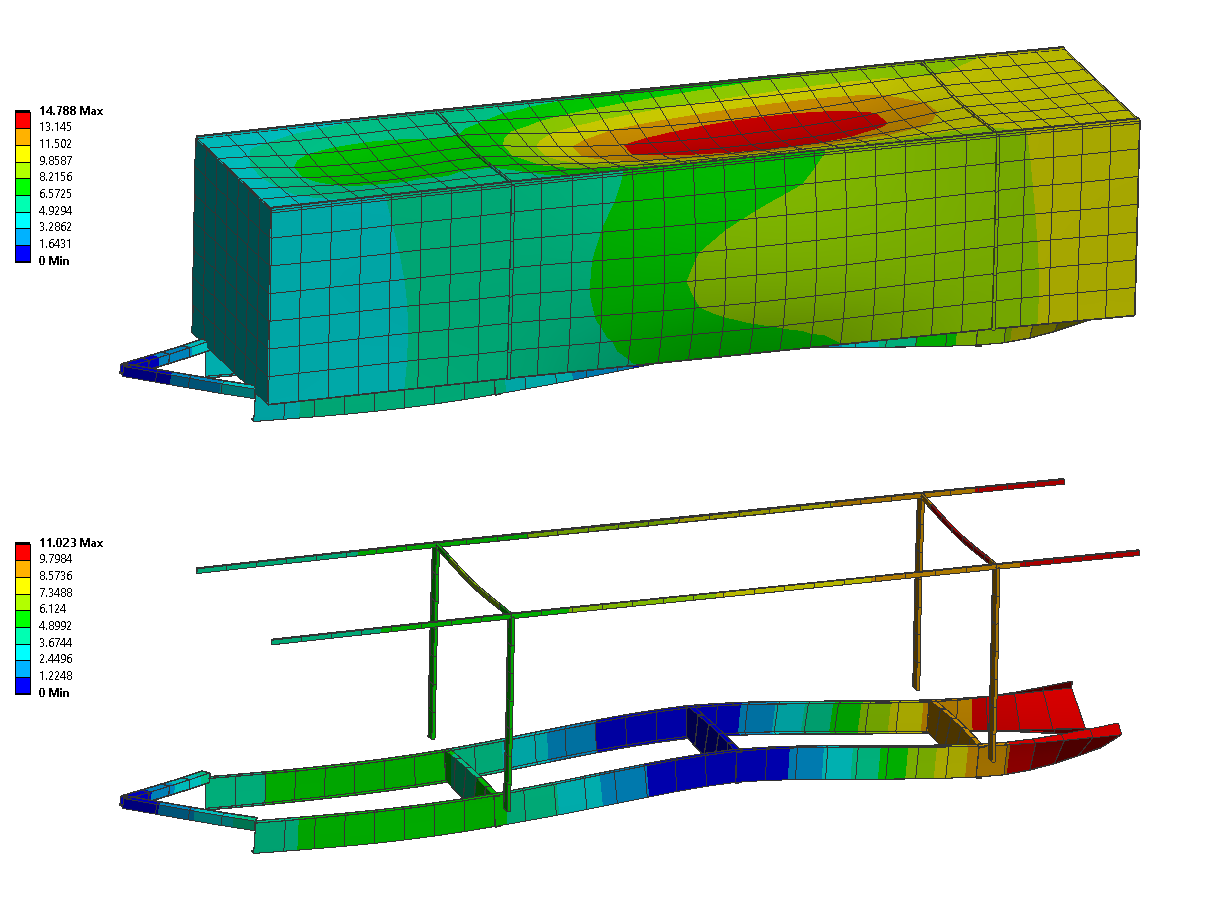
\includegraphics[width=1\linewidth]{04_figures/FEM 1.1.png}
  \caption{Verformung des Solar Butterflys im Lastfall der vertikalen Beschleunigung}
  \label{FEM 1.1}
\end{figure}


\newpage

\subsubsection{Laterale Beschleunigung}
\begin{table}[H]
\centering
\begin{tabular}{lcccccc}
Grösse	&	Einheit	&	x	&	y	&	z	&	Total	&	Berechnet	\\	\hline
\multicolumn{5}{l}{\textbf{Lagerreaktionen}}									&		&		\\	\thickhline
Deichsel	&	N	&	-20611	&	-3050	&	0	&	20835	&	206000	\\
Chassis Links	&	N	&	0	&	1525	&	515	&	1610	&		\\
Chassis Rechts	&	N	&	0	&	1525	&	-515	&	1610	&		\\	\hline	\\
\multicolumn{5}{l}{\textbf{Chassis}}									&		&		\\	\thickhline
Axialkraft	&	N	&		&		&		&	6080	&		\\
Querkraft	&	N	&		&		&		&	1319	&	 \\
Biegemoment	&	kNmm	&		&		&		&	2601	&		\\	\hline	\\
\multicolumn{5}{l}{\textbf{Dach}}									&		&		\\	\thickhline
Axialkraft	&	N	&		&		&		&	553	&		\\
Querkraft	&	N	&		&		&		&	8	&		\\
Biegemoment	&	kNmm	&		&		&		&	2	&		\\	\hline	\\
\multicolumn{5}{l}{\textbf{Träger A und B}}													\\	\thickhline
Axialkraft	&	N	&		&		&		&	-1562	&		\\
Querkraft	&	N	&		&		&		&	56	&		\\
Biegemoment	&	kNmm	&		&		&		&	17	&		\\	\hline	\\
\multicolumn{5}{l}{\textbf{Kontaktreaktion: Chassis - Träger A und B}}									&		&		\\	\thickhline
 Axialkraft A	&	N	&	-56	&	2084	&	325	&	2110	&		\\
Biegemoment A	&	kNmm	&	-734	&	-19	&	2	&	734	&		\\
Axialkraft B	&	N	&	98	&	667	&	80	&	679	&		\\
Biegemoment B	&	kNmm	&	-236	&	34	&	-14	&	238	&		\\	\hline	\\
\multicolumn{5}{l}{\textbf{Kontaktreaktion: Chassis - Boden}}									&		&		\\	\thickhline
Normalkraft (Zug)	&	N	&		&		&		&	35	&		\\
Schubkraft (xz-Ebene)	&	N	&		&		&		&	1733	&		\\	\hline
\end{tabular}
\caption{Resultate der FEM-Simulation des Lastafalles der lateralen Beschleunigung}
\label{tab:FEM 1.2}
\end{table}


\begin{figure}[H]
  \centering
  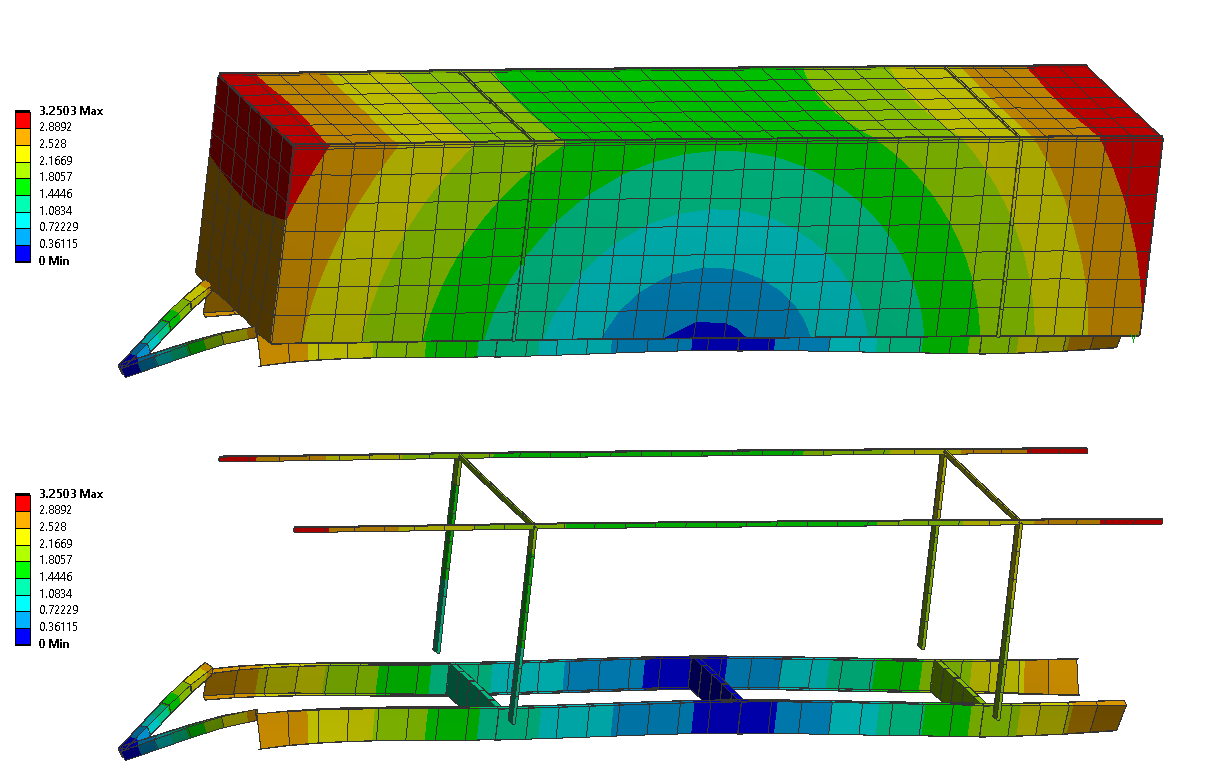
\includegraphics[width=1\linewidth]{04_figures/FEM 1.2.png}
  \caption{Verformung des Solar Butterflys im Lastfall der lateralen Beschleunigung}
  \label{FEM 1.2}
\end{figure}

\subsubsection{Longitudinale Beschleunigung}
\begin{table}[H]
\centering
\begin{tabular}{lcccccc}
Grösse	&	Einheit	&	x	&	y	&	z	&	Total	&	Berechnet	\\	\hline
\multicolumn{5}{l}{\textbf{Lagerreaktionen}}									&		&		\\	\thickhline
Deichsel	&	N	&	0	&	0	&	1023	&	1023	&	-330	\\
Chassis Links	&	N	&	0	&	-15008	&	11290	&	18780	&	11900	\\
Chassis Rechts	&	N	&	0	&	15008	&	11242	&	18752	&	11900	\\	\hline	\\
\multicolumn{5}{l}{\textbf{Chassis}}									&		&		\\	\thickhline
Axialkraft	&	N	&		&		&		&	-31674	&	-11480	\\
Querkraft	&	N	&		&		&		&	7163	&	6100	\footnotemark \\
Biegemoment	&	kNmm	&		&		&		&	6658	&		\\	\hline	\\
\multicolumn{5}{l}{\textbf{Dach}}									&		&		\\	\thickhline
Axialkraft	&	N	&		&		&		&	-2560	&	-964	\\
Querkraft	&	N	&		&		&		&	24	&		\\
Biegemoment	&	kNmm	&		&		&		&	13	&		\\	\hline	\\
\multicolumn{5}{l}{\textbf{Träger A und B}}													\\	\thickhline
Axialkraft	&	N	&		&		&		&	2684	&		\\
Querkraft	&	N	&		&		&		&	1067	&		\\
Biegemoment	&	kNmm	&		&		&		&	627	&		\\	\hline	\\
\multicolumn{5}{l}{\textbf{Kontaktreaktion: Chassis - Träger A und B}}									&		&		\\	\thickhline
 Axialkraft A	&	N	&	237	&	-3577	&	1729	&	3979	&		\\
Biegemoment A	&	kNmm	&	1924	&	71	&	-102	&	1928	&		\\
Axialkraft B	&	N	&	-733	&	-4221	&	1679	&	4602	&		\\
Biegemoment B	&	kNmm	&	2097	&	-251	&	95	&	2114	&		\\	\hline	\\
\multicolumn{5}{l}{\textbf{Kontaktreaktion: Chassis - Boden}}									&		&		\\	\thickhline
Normalkraft (Zug)	&	N	&		&		&		&	1942	&		\\
Schubkraft (xz-Ebene)	&	N	&		&		&		&	10972	&		\\	\hline
\end{tabular}
\caption{Resultate der FEM-Simulation des Lastafalles der longitudinalen Beschleunigung}
\label{tab:FEM 1.4}
\end{table}
\footnotetext[3]{Unter der Annahme, dass nur das Chassis Querkräfte aufnimmt. Die Kraft von 6.1 kN ergibt sich aus der Halbierung der globalen Querkraft aus der Berechnung im Kapitel \ref{1.4 Laterale Beschleunigung}.}



\begin{figure}[H]
  \centering
  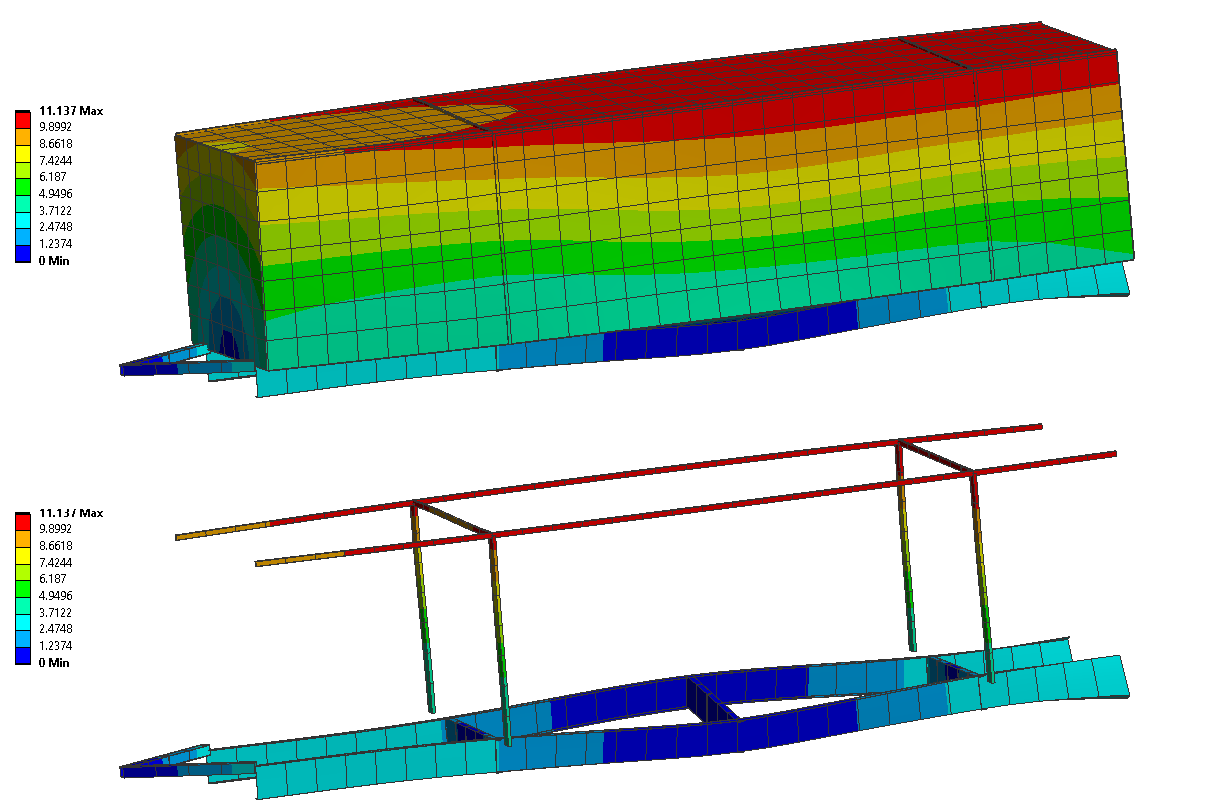
\includegraphics[width=1\linewidth]{04_figures/FEM 1.4.png}
  \caption{Verformung des Solar Butterflys im Lastfall der longitudinalen Beschleunigung}
  \label{FEM 1.4}
\end{figure}

\subsubsection{Rotatorische Beschleunigung}
\begin{table}[H]
\centering
\begin{tabular}{lcccccc}
Grösse	&	Einheit	&	x	&	y	&	z	&	Total	&	Berechnet	\\	\hline
\multicolumn{5}{l}{\textbf{Lagerreaktionen}}									&		&		\\	\thickhline
Deichsel	&	N	&	0	&	0	&	804	&	804	&		\\
Chassis Links	&	N	&	0	&	-23097	&	10913	&	25546	&	-27000	\footnotemark \\
Chassis Rechts	&	N	&	0	&	23097	&	10844	&	25516	&	27000	\\	\hline	\\
\multicolumn{5}{l}{\textbf{Chassis}}									&		&		\\	\thickhline
Axialkraft	&	N	&		&		&		&	44164	&		\\
Querkraft	&	N	&		&		&		&	10927	&		\footnotemark \\
Biegemoment	&	kNmm	&		&		&		&	10218	&		\\	\hline	\\
\multicolumn{5}{l}{\textbf{Dach}}									&		&		\\	\thickhline
Axialkraft	&	N	&		&		&		&	3625	&		\\
Querkraft	&	N	&		&		&		&	32	&		\\
Biegemoment	&	kNmm	&		&		&		&	19	&		\\	\hline	\\
\multicolumn{5}{l}{\textbf{Träger A und B}}													\\	\thickhline
Axialkraft	&	N	&		&		&		&	4119	&		\\
Querkraft	&	N	&		&		&		&	1311	&		\\
Biegemoment	&	kNmm	&		&		&		&	772	&		\\	\hline	\\
\multicolumn{5}{l}{\textbf{Kontaktreaktion: Chassis - Träger A und B}}									&		&		\\	\thickhline
 Axialkraft A	&	N	&	373	&	-5525	&	2346	&	6014	&		\\
Biegemoment A	&	kNmm	&	2767	&	112	&	-164	&	2774	&		\\
Axialkraft B	&	N	&	-1309	&	-6399	&	2221	&	6899	&		\\
Biegemoment B	&	kNmm	&	2996	&	-452	&	159	&	3034	&		\\	\hline	\\
\multicolumn{5}{l}{\textbf{Kontaktreaktion: Chassis - Boden}}									&		&		\\	\thickhline
Normalkraft (Zug)	&	N	&		&		&		&	3118	&		\\
Schubkraft (xz-Ebene)	&	N	&		&		&		&	10761	&		\\	\hline
\end{tabular}
\caption{Resultate der FEM-Simulation des Lastafalles der rotatorischen Beschleunigung}
\label{tab:FEM 1.5}
\end{table}

\footnotetext[4]{Die Kräfte von  $\pm$ 27 kN ergeben sich aus der Halbierung der Kraft F aus der Berechnung im Kapitel \ref{1.5 Rotatorische Beschleunigung}.}

\begin{figure}[H]
  \centering
  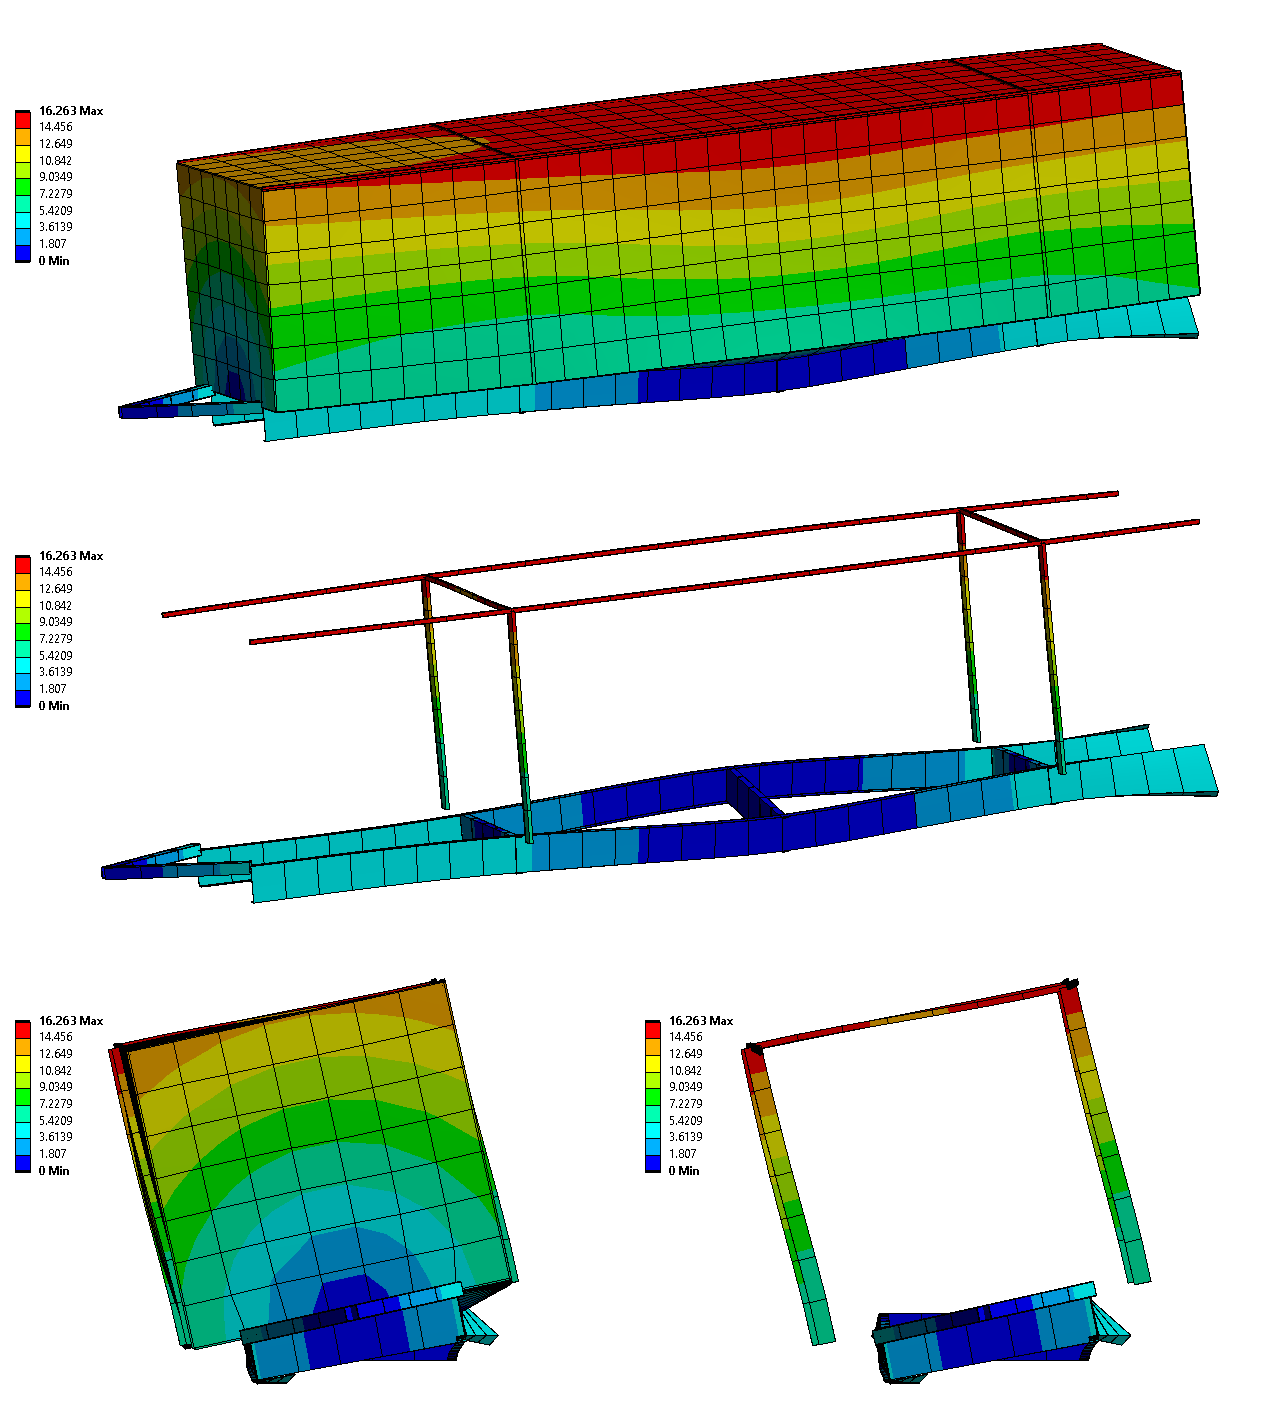
\includegraphics[width=1\linewidth]{04_figures/FEM 1.5.png}
  \caption{Verformung des Solar Butterflys im Lastfall der rotatorischen Beschleunigung}
  \label{FEM 1.5}
\end{figure}


\newpage
